%%%%%%%%%%%%%%%%%%%%%%%%%%%%%%%%%%%%%%%%%
% University/School Laboratory Report
% LaTeX Template
% Version 3.1 (25/3/14)
%
% This template has been downloaded from:
% http://www.LaTeXTemplates.com
%
% Original author:
% Linux and Unix Users Group at Virginia Tech Wiki 
% (https://vtluug.org/wiki/Example_LaTeX_chem_lab_report)
%
% License:
% CC BY-NC-SA 3.0 (http://creativecommons.org/licenses/by-nc-sa/3.0/)
%
%%%%%%%%%%%%%%%%%%%%%%%%%%%%%%%%%%%%%%%%%

\documentclass{article}

%\usepackage[version=3]{mhchem} % Package for chemical equation typesetting
%\usepackage{siunitx} % Provides the \SI{}{} and \si{} command for typesetting SI units
\usepackage{graphicx} % Required for the inclusion of images
\usepackage{natbib} % Required to change bibliography style to APA
\usepackage{amsmath} % Required for some math elements 
\usepackage{listings}
\lstset{basicstyle=\ttfamily, breaklines=true}
\setlength\parindent{2pt} % Removes all indentation from paragraphs
\linespread{1.5}
%\renewcommand{\labelenumi}{\alph{enumi}.} % Make numbering in the enumerate environment by letter rather than number (e.g. section 6)

%\usepackage{times} % Uncomment to use the Times New Roman font


%----------------------------------------------------------------------------------------
%	DOCUMENT INFORMATION
%----------------------------------------------------------------------------------------

\title{Exam test\\UML for Embedded Systems} % Title

\author{Simone \textsc{Rossi}} % Author name

\date{\today} % Date for the report

\begin{document}

\maketitle % Insert the title, author and date

\begin{center}
\begin{tabular}{l r}
Date Performed: & \today \\ % Date the experiment was performed
Partners: & Simone Rossi \\ % Partner names
%& Mary Smith \\
%Instructor: & Professor Smith % Instructor/supervisor
\end{tabular}
\end{center}

% If you wish to include an abstract, uncomment the lines below
% \begin{abstract}
% Abstract text
% \end{abstract}

%----------------------------------------------------------------------------------------
%	SECTION 1
%----------------------------------------------------------------------------------------

\section{Assumptions}
\begin{figure}[h!]
  \centering
  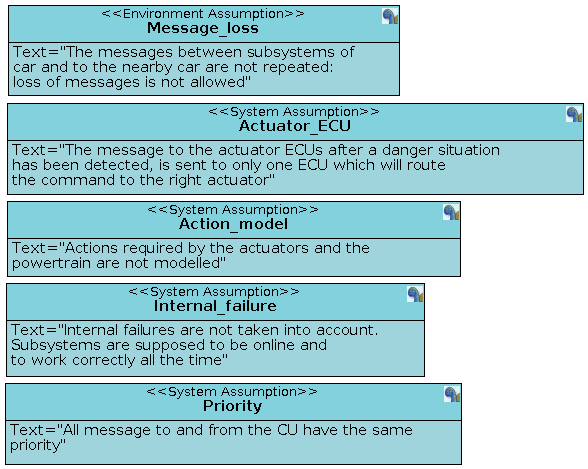
\includegraphics[width = 0.8\textwidth]{./assumptions.png}
\end{figure}

\section{Formal verification}

For the formal verificaton, I checked that in all dangerous situations a broadcast message is sent to the nearby cars. To do that, I proved the reachability and the liveness properties of the "message broadcast send" action in the CU are guaranteed. \\

The formal verification confirmed that these two properties are verified; this means that a message is always sent whenever a dangerous situation has been detected. \\

Morover, I checked that the maximum time delay from the moment in which a dangerous situation has occurred and a broadcast message is sent is not more than 150 ms. To do that, I introduced an observer to between the \texttt{Sensor Chassis ECU} and the \texttt{CU}. Using a timer, I formally proved that the message is sent within 150 ms (e.g. the timer never expires and that state is never reachable).\\

\begin{figure}[h!]
  \centering
  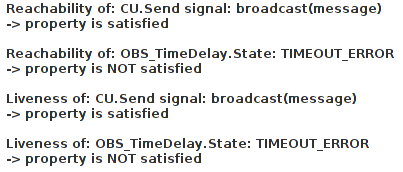
\includegraphics[width = \textwidth]{./formal.png}
\end{figure}
\end{document}
